\documentclass[11pt]{article}
\usepackage{palatino,graphicx}
\pagestyle{headings}

\def\hdr {{\parindent 0pt  \vskip -0.7in%
EE369C  Fall 2017-18 \hfill \\
Medical Image Reconstruction \hfill  \\
\vskip 0.1in }}

\frenchspacing

\topmargin=-0.5in
\textheight=9in
\evensidemargin 0.0in
\oddsidemargin 0.0in
\setlength{\textwidth}{6.5in}

\begin{document}
\
\hdr


\begin{center}
{\Large\em EE369C:  Assignment 3} \\[0.15in]
{\em Due Wednesday, Oct 18}
\end{center}

This assignment shows how to do off-resonance correction for spiral k-space trajectories. 
The data set for this assignment is a pretty shot of a GE resolution phantom
\begin{quote}
 {\tt http://www.stanford.edu/class/ee369c/data/resphantom2.mat}. 
\end{quote}
This includes two full data sets at two different echo times.  This will allow you to compute full resolution field maps, that you will use for map based off-resonance correction.  Note that the data set is inverted and flipped when directly reconstructed.  You can leave it this way, or orient it as you see it here, as you wish.

The data sets are in the matlab variables \verb+d1+ and \verb+d2+.  Each has 2048 samples per spiral readout, and 16 readouts per scan.  The duration of each readout is 8.192 ms.  The echo times for each data set are in the matlab variables \verb+te1+ and \verb+te2+. The k-space trajectory is stored in \verb+ks+ and the density precompensation in \verb+wt+.  The data should reconstruct to a 160x160 image. 

A reconstruction of the data set is shown in Fig.~\ref{im1}.  While this isn't too bad an image, it is clear that it could use some help. Parts of the image are blurred due to local off-resonance frequency shifts.  In this assignment we will first make a map of the frequency shifts.  Then, generate a multifrequency reconstruction (using your gridding code from the last assignment).  Then, you'll do a map based reconstruction, and an autofocus reconstruction.  

\begin{figure}[bh]
  \begin{center}
  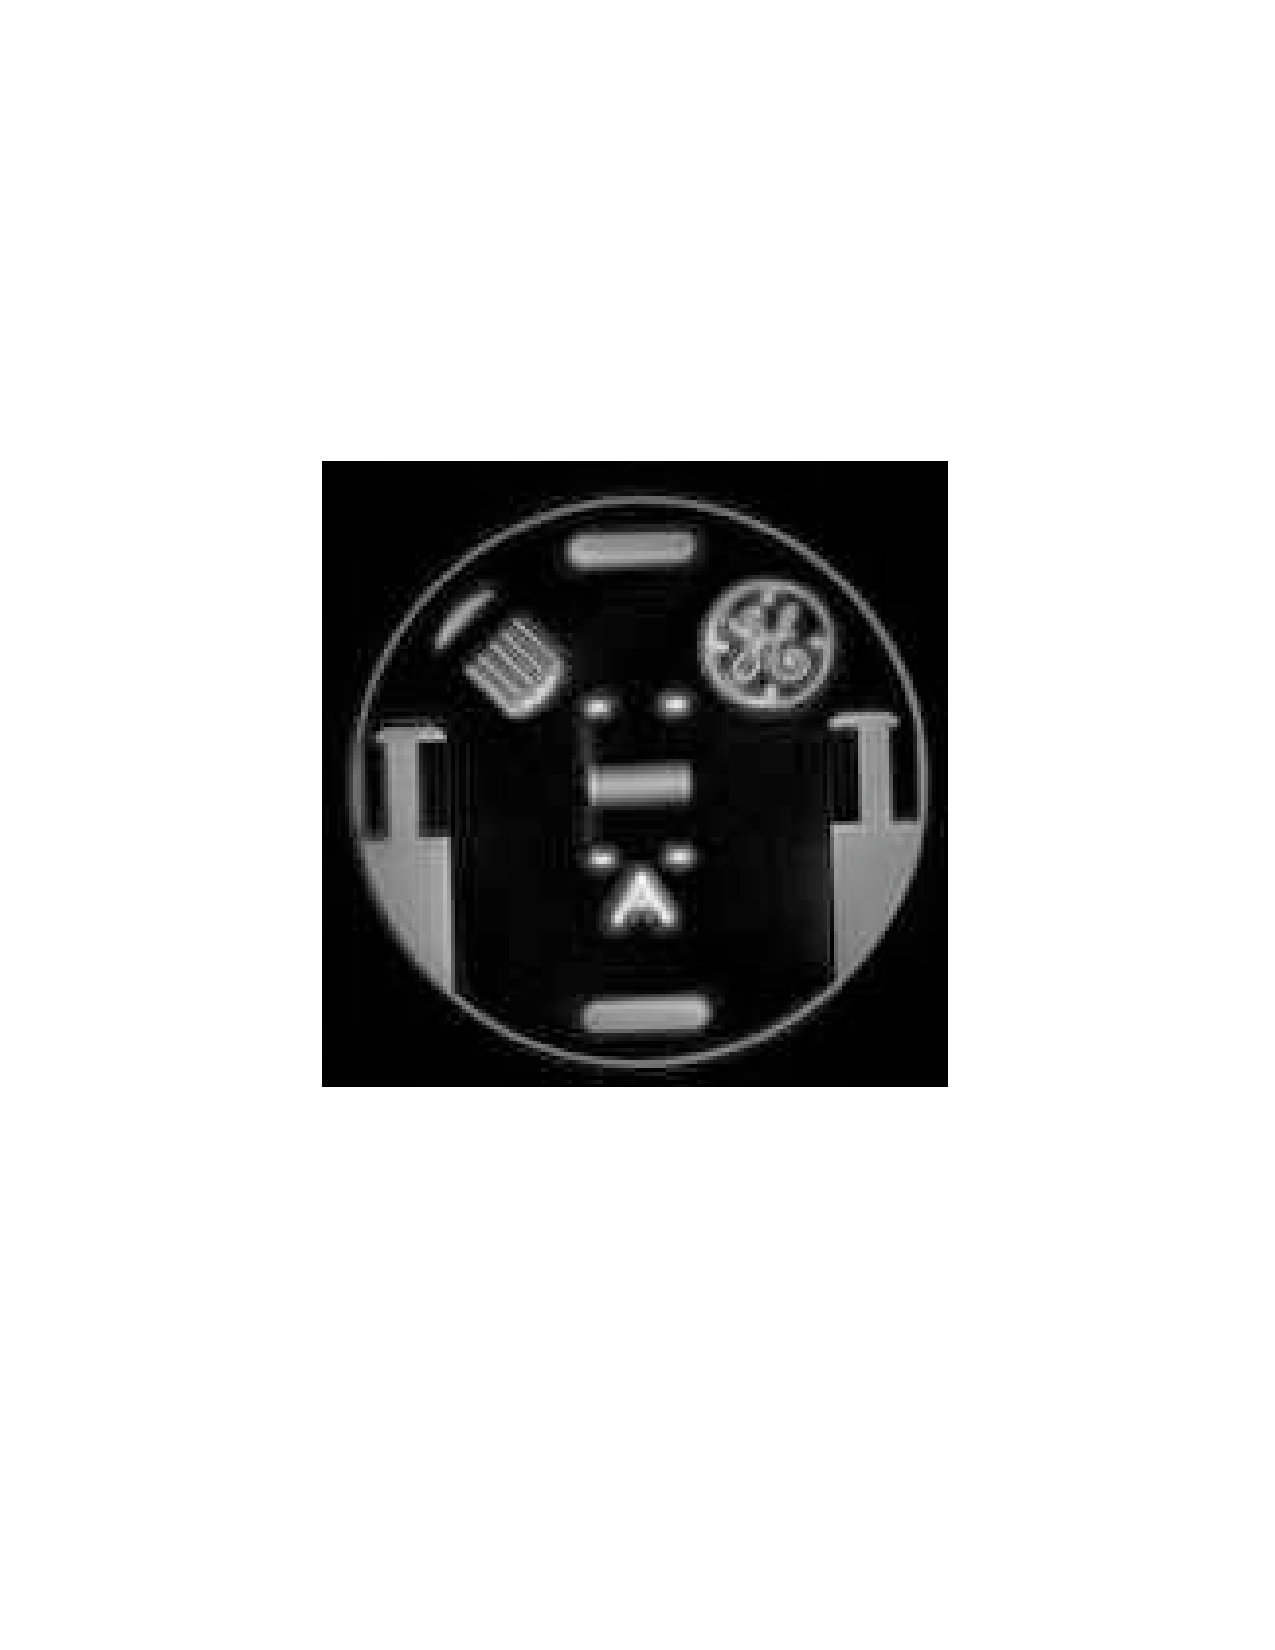
\includegraphics[width=2.5in]{im1w0.pdf}
  \end{center}
  \caption[]{Simple reconstruction of the first data set. While much of the image is in focus, note the blurring around the resolution comb, and the GE logo.}
  \label{im1}
\end{figure}


\paragraph*{\bf 1. Field Map}

Reconstruct each of the data sets using your gridding reconstruction.  If you are unsure of your implementation, use \verb+gridkb.m+ from the course web page.  Note that \verb+gridkb.m+ can return either the image or the k-space data, which may be useful below.  Display the two reconstructions.

From the two data sets, compute a field map measured in Hz. Display the field map.   If we limit our attention to pixels whose amplitude are  greater than 10\% of the maximum, what range of frequencies do you observe?  You may find it useful to implement this as an m-file that takes two images, and returns the field map
\begin{verbatim}
>> fm = compute_fm(im1,te1,im2,te2)
\end{verbatim}

\paragraph*{2. Multifrequency Reconstruction}

Write an m-file that takes a data set, and returns reconstructions over a set of frequencies,
\begin{verbatim}
>> im_mf = mf_recon(d, k, w, n, te, tad, fmin, fmax, fstep)
\end{verbatim}
where \verb+d+ is the acquired data, \verb+k+ is the k-space trajectory, \verb+w+ is the preweighting, and \verb+n+ is the image size, as usual.  The reconstruction is performed starting at \verb+fmin+, and goes to \verb+fmax+ in steps of \verb+fstep+ Hz.   Note that the echo time is required, \verb+te+, as is the A/D time \verb+tad+.  The time of each sample during the acquisition is then
\begin{verbatim}
>>  [ns ni] = size(d);
>>  t = te + [0:ns-1]*tad/ns;
\end{verbatim}
This includes the phase evolution during the time between the RF pulse and the start of the acquisition.

Your reconstruction will return a 3D array  \verb+im_fm(n,n,nf)+ where \verb+nf+ is the number of frequency steps from \verb+fmin+ to \verb+fmax+.

Your reconstruction can either use the simple approach of doing the full gridding reconstruction of
\begin{verbatim}
>> d.*exp(-i*2*pi*f*t)
\end{verbatim}
for each frequency \verb+f+, or it can be more efficient, and grid once, and multiply by a phase function in k-space as we talked about in class (the discrete frequency reconstruction).

Reconstruct the first data set for \verb+f+ equal to  -128 Hz to 128 Hz in steps of 16 Hz.  128 Hz is one cycle over the readout duration.  The step size is smaller than we need by a factor of two.  Show reconstructions at -128 Hz, -64 Hz, 64 Hz, and 128 Hz.  The 0 Hz reconstruction should look like Fig.~\ref{im1}.  Go through the set interactively, and note what frequencies different parts of the image come into focus.  This will help you debugging the next part.

\paragraph*{3. Field Map Based Reconstruction}

The field map tells you the frequency  (in Hz) of each voxel.  Use that to choose a reconstruction from the multifrequency reconstruction on a pixel-by-pixel basis.  Display your result. Where do you see artifacts?

{\em Hint: } This should look much better!  If not, check to see if you have the sign of the frequency shift switched.


\paragraph*{4. Autofocus Reconstruction}

Finally, we'll look at an autofocus reconstruction.   Essentially, what we want to do is automatically choose one of the multi-frequency reconstructions based on a focus metric.

\subparagraph{a) Phase Correction} 
Since we are counting on the off-resonance phase to produce an imaginary image component, we need to correct for the constant image phase.  We'll do this by computing a low resolution reconstruction (instantaneous in time) for each frequency.  We use the multifrequency reconstruction you wrote above, but just using the first 1 ms of data (256 samples, 1/8 of the total data) 
\begin{verbatim}
>> im_r=mf_recon(d1(1:256,:),k(1:256,:),w(1:256,:),n,te,tad/8,fmin,fmax,fstep);
\end{verbatim}
The phase correction is then
\begin{verbatim}
>> pc = exp(-i*angle(im_r));
\end{verbatim}
We are going to use the absolute value of the imaginary part of the phase corrected reconstruction as a focus metric.  If \verb+im_mf+ is the multifrequency reconstruction of data set 1, display
\begin{verbatim}
>> imshow(abs(imag(im_mf(:,: n).*pc(:,:,n))),[])
\end{verbatim}
for n corresponding to f = -64 Hz,  0 Hz,  and 64 Hz.  Does the focus metric decrease when the frequency is correct?


\subparagraph*{b) Focus Metric}
The focus metric is the absolute value of the phase corrected imaginary component, integrated over a local window.  The absolute value of the phase corrected imaginary component is
\begin{verbatim}
>> fc = abs(imag(im_mf.*pc)))
\end{verbatim}
For each frequency, we can integrate over a 5x5 window by
\begin{verbatim}
>> fcf = 0*fc;
>> for n = 1:nf,
>>   fcf(:,:,n) = conv2(fc(:,:,n), ones(5,5)/25, 'same');
>> end;
\end{verbatim}
This integrates over a 5x5 widow, registered with the original data. Display the filtered \verb+fcf+ for f = -64 Hz, 0 Hz, and 64 Hz.

\subparagraph{c)  Autofocus Reconstruction}
For each pixel, choose the reconstruction with the smallest focus metric.  Keep track of both the reconstruction, and the index of the frequency that was chosen. This is a field map derived from the data itself.  Display the autofocus reconstruction and the field map. 

This should look pretty good, but not perfect.  What simple thing can you do to fix it? Describe your fix, and show the improved reconstruction and field map.

\vspace{0.125in}
{\em Hint:} Do you need +/- 128 Hz frequency range?  What does too big a range do?





\end{document}

